\section{Generative Adversarial Networks } \label{sec:gan}

The main reference for this paper is from \cite{zou2019}. We begin by motivating the methodology with a typical problem facing remote sensing images. Typically, images captured from satellites orbiting earth are attenuated by cloud covering making the information retrieval used in various applications challenging. Therefore, the research on cloud detection and its subsequent removal from images has received significant amount of attention in recent years \textcolor{red}{(add citation and further elaboration?)}. 

Although most of the research frame this problem as a pixel-level classification problem \textcolor{red}{(add citation)}, pixel-wise classification leads to category ambiguity for detection of semi-transparent clouds. In other words, the cloud probability output from convolutional networks for each pixel are often inconclusive for areas of the image covered by semi-transparent clouds. Recognizing this issue, the authors of \cite{zou2019} recast the problem as mixed energy separation problem commonly referred to as image matting. As illustrated in Figure \ref{fig:image_matting}, the main assumption is that the energy received at the sensor $\varepsilon_{sensor}$ is a linear combination the energy reflected from clouds $\varepsilon_{c}$ and 

\begin{figure}[h]
\centering
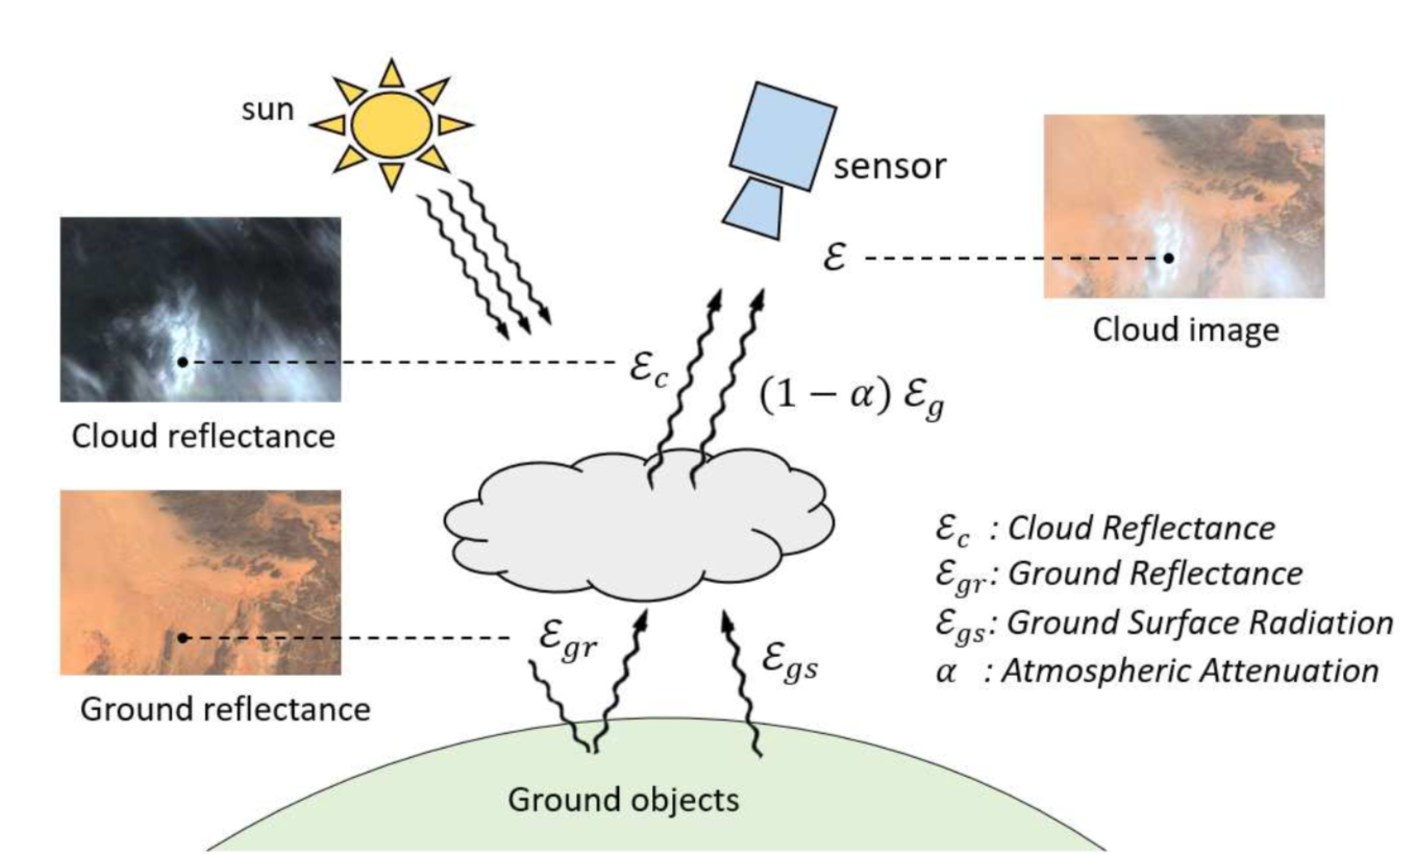
\includegraphics[width=0.75\textwidth]{images/cloud_matting_image}
\caption{Imaging model of cloud images.}
\label{fig:image_matting}
\end{figure}